\documentclass[conference]{IEEEtran}
\usepackage[utf8]{inputenc}
\usepackage[spanish,english]{babel}
\usepackage{graphicx}
\usepackage{float}

\begin{document}

\title{Arquitectura de Software, Patrones de Diseño y Metodologías Ágiles}

\author{
    \IEEEauthorblockN{Yordy Erik Nuñez Pineda, Jesús Ariel González Bonilla}
    \IEEEauthorblockA{
        \textit{Servicio Nacional de Aprendizaje SENA} \\
        yordierik05@gmail.com, jagonzalezb@sena.edu.co
    }
}

\maketitle

\begin{abstract}
This article explores the intersection between software architecture, design patterns, and agile methodologies, highlighting their importance as essential tools to address the challenges of developing complex systems. A comprehensive review of various approaches is provided, emphasizing the benefits of integrating agile methodologies, such as SCRUM, XP, and TDD, with robust architectures, such as microservices, hexagonal architecture, and the 4+1 model. Furthermore, the fundamental role of design patterns in creating sustainable and reusable systems, thereby improving software quality, is examined. Through a comparative analysis of studies and case studies, the article proposes a conceptual framework that combines these disciplines, promoting scalability, adaptability, and quality in modern software projects. Special attention is paid to applications in distributed, mobile, and enterprise systems, offering a comprehensive approach that benefits development teams in their search for effective solutions.\\
\end{abstract}

\begin{IEEEkeywords}
Software Architecture, Design Patterns, Microservices, Sustainability, Scalability, Agile Methodologies.\\
\end{IEEEkeywords}

\begin{otherlanguage}{spanish}
\begin{abstract}
Este artículo explora la intersección entre la arquitectura de software, los patrones de diseño y las metodologías ágiles, destacando su importancia como herramientas esenciales para abordar los desafíos del desarrollo de sistemas complejos. Se realiza una revisión exhaustiva de diversos enfoques, enfatizando los beneficios de integrar metodologías ágiles, como SCRUM, XP y TDD, con arquitecturas robustas, tales como microservicios, arquitectura hexagonal y el modelo 4+1. Además, se examina el papel fundamental de los patrones de diseño en la creación de sistemas sostenibles y reutilizables, lo que mejora la calidad del software. A través de un análisis comparativo de estudios y casos prácticos, el artículo propone un marco conceptual que combina estas disciplinas, promoviendo la escalabilidad, adaptabilidad y calidad en proyectos de software modernos. Se presta especial atención a las aplicaciones en sistemas distribuidos, móviles y empresariales, ofreciendo un enfoque integral que beneficia a los equipos de desarrollo en su búsqueda de soluciones efectivas.\\
\end{abstract}

\begin{IEEEkeywords}
Arquitectura de Software, Patrones de Diseño, Microservicios, Sostenibilidad, Escalabilidad, Metodologías Ágiles.
\end{IEEEkeywords}
\end{otherlanguage}

\section{Introducción}
En las últimas décadas, el desarrollo de software ha experimentado una transformación profunda debido a la creciente demanda de sistemas más rápidos, escalables y adaptables. Estas necesidades han llevado a la consolidación de tres pilares esenciales: la arquitectura de software, los patrones de diseño y las metodologías ágiles. Cada uno de estos elementos juega un papel fundamental en la creación de soluciones robustas y sostenibles, pero su integración efectiva aún representa un desafío significativo para los equipos de desarrollo.\\

La creciente complejidad de los sistemas modernos, que abarcan desde aplicaciones móviles hasta sistemas distribuidos y empresariales, ha puesto de manifiesto las limitaciones de enfoques tradicionales en el desarrollo de software. Por un lado, la falta de planificación arquitectónica en metodologías ágiles puede comprometer la calidad estructural de los sistemas, dificultando su mantenimiento y escalabilidad. Por otro lado, la implementación de patrones de diseño y arquitecturas robustas suele percibirse como incompatible con la velocidad y flexibilidad que demandan los proyectos ágiles. Esto genera una dicotomía entre la adaptabilidad y la sostenibilidad, que, si no se aborda adecuadamente, puede derivar en altos costos de mantenimiento y baja calidad del producto final.\\

El objetivo de este artículo es proponer un marco conceptual que combine la arquitectura de software, los patrones de diseño y las metodologías ágiles para resolver los desafíos mencionados. Este marco busca integrar los principios de modularidad y escalabilidad de arquitecturas modernas, como los microservicios y la arquitectura hexagonal, con la flexibilidad y eficiencia de metodologías ágiles como SCRUM y XP. Además, se propone el uso de patrones de diseño y técnicas como el desarrollo dirigido por pruebas (TDD) para garantizar la calidad del software desde las etapas iniciales del desarrollo.\\

La integración de estos enfoques no solo es necesaria para afrontar los retos técnicos de proyectos modernos, sino que también es crucial para mejorar la colaboración y comunicación entre los \textit{stakeholders}. En un contexto en el que los equipos de desarrollo trabajan en entornos altamente dinámicos, contar con una base arquitectónica sólida y patrones de diseño bien definidos puede facilitar la adaptabilidad a cambios, la identificación de problemas y la implementación de soluciones rápidas. Este artículo reúne aportes teóricos y prácticos de múltiples investigaciones, ofreciendo una guía que puede ser aplicada tanto en entornos empresariales como académicos.\\

El marco conceptual propuesto está diseñado para ser aplicable en diversos contextos, desde proyectos de pequeña escala hasta sistemas distribuidos de alta complejidad. Se exploran casos prácticos y estudios que demuestran cómo la documentación adecuada, la modularidad y la aplicación de patrones mejoran la calidad y reducen los costos asociados al desarrollo de software.\\

Con este planteamiento, el artículo busca sentar las bases para un enfoque más integrado y sostenible, permitiendo a los equipos de desarrollo enfrentar los desafíos contemporáneos con soluciones más efectivas y adaptables.\\

\section{Marco Teórico}
El marco teórico de este artículo se centra en tres áreas fundamentales para el desarrollo de software contemporáneo: la arquitectura de software, los patrones de diseño y las metodologías ágiles. Estas disciplinas se entrelazan para ofrecer soluciones robustas, adaptables y sostenibles en un entorno de constante evolución tecnológica. A continuación, se presentan los conceptos, teorías y estudios previos que sustentan la integración de estos enfoques en proyectos de software modernos.\\

\subsection{Arquitectura de Software}
La arquitectura de software es la disciplina que define la estructura, el comportamiento y la interacción de los componentes de un sistema. Según el modelo 4+1 de Philippe Kruchten, la arquitectura se documenta a través de múltiples vistas que representan aspectos esenciales del sistema: lógica, procesos, desarrollo, implementación y escenarios. Este enfoque permite descomponer sistemas complejos en módulos independientes, facilitando su comprensión y mantenimiento.\\

Por otra parte, la arquitectura hexagonal, propuesta por Alistair Cockburn, destaca la importancia de separar la lógica del negocio de las tecnologías externas mediante el uso de puertos y adaptadores. Esto fomenta la modularidad y asegura que los sistemas sean independientes de las herramientas tecnológicas, lo que facilita su evolución.\\

En aplicaciones modernas, como los sistemas distribuidos, los microservicios han ganado popularidad. Esta arquitectura divide los sistemas en pequeños servicios independientes que se comunican mediante APIs, lo que mejora la escalabilidad y permite el desarrollo paralelo por equipos. Los estudios revisados destacan casos como la Asamblea Nacional del Ecuador, donde los microservicios facilitaron el mantenimiento de aplicaciones complejas, y el Banco de la República de Colombia, que utilizó un modelo SOA para gestionar servicios de seguridad PKI.\\

\subsection{Patrones de Diseño}
Los patrones de diseño son soluciones probadas a problemas comunes en el desarrollo de software, formalizadas por autores como la "Gang of Four" (GoF). Patrones como el Observador, el MVC y la Factoría Abstracta se han consolidado como herramientas clave para mejorar la sostenibilidad y reutilización del código.\\

El patrón MVC, por ejemplo, separa la lógica de negocio de la presentación y la interacción, facilitando la actualización independiente de cada capa. Este enfoque ha sido ampliamente adoptado en aplicaciones web y móviles, como se evidenció en el estudio de la Universidad del Quindío sobre arquitecturas móviles. Por su parte, el patrón Observador permite a los componentes del sistema reaccionar automáticamente a cambios en otros, favoreciendo la interacción dinámica en entornos distribuidos.\\

Los patrones de diseño no solo estructuran los sistemas, sino que también mejoran su calidad y mantenimiento. Sin embargo, estudios previos destacan que su implementación en entornos ágiles requiere considerar la testeabilidad y la integración con metodologías como TDD. En este contexto, el artículo "Calidad Ágil" analiza cómo los patrones pueden integrarse en flujos de desarrollo dirigidos por pruebas, asegurando que cumplan con requisitos de encapsulación y cohesión.\\

Además, se han desarrollado enfoques educativos, como el juego "Coffee Challenge", para enseñar patrones de diseño a estudiantes, lo que demuestra su importancia en la formación de ingenieros y su impacto en la práctica profesional.\\

\subsection{Metodologías Ágiles}
Las metodologías ágiles, como SCRUM, XP y TDD, priorizan la adaptabilidad y la entrega continua de valor en ciclos cortos. Sin embargo, su implementación a menudo descuida la planificación arquitectónica, lo que puede comprometer la sostenibilidad del sistema. Para abordar esta limitación, se han propuesto soluciones como el Sprint 0, un ciclo inicial en SCRUM destinado a diseñar la arquitectura preliminar.\\

El desarrollo dirigido por pruebas (TDD) complementa estas metodologías al asegurar la calidad del software desde las primeras etapas. En TDD, las pruebas se escriben antes del código, lo que permite verificar que cada componente cumple con su función antes de integrarse en el sistema. Estudios previos, como el caso del Sistema Automático de Control de Velocidad (SCACV), han demostrado cómo TDD puede aplicarse en conjunto con patrones de diseño, mejorando la modularidad y la eficiencia del desarrollo.\\

Otro enfoque interesante es el uso de ICONIX, una metodología que combina elementos ágiles con un proceso más estructurado, permitiendo documentar y validar la arquitectura en etapas tempranas. Este método se ha utilizado con éxito en la integración de arquitecturas y metodologías ágiles en sistemas empresariales, mostrando cómo es posible equilibrar la flexibilidad y la planificación.\\

\subsection{Documentación y Calidad}
La documentación adecuada de la arquitectura es crucial para la trazabilidad y el mantenimiento de sistemas complejos. Modelos como \textit{``Vistas y más allá''} del SEI y el estándar IEEE 1471 destacan la importancia de adaptar la documentación a las necesidades de los \textit{stakeholders}. Esto incluye la creación de plantillas para cada vista arquitectónica, asegurando consistencia y claridad en el diseño.\\

El uso de herramientas como \textit{SonarQube} y frameworks UML también se ha destacado en los estudios revisados como estrategias efectivas para evaluar métricas de calidad y modelar patrones de diseño. Estas prácticas no solo mejoran la comprensión del sistema, sino que también facilitan su evolución en contextos dinámicos.\\

\subsection{Integración de Enfoques}
La convergencia de estas disciplinas permite desarrollar sistemas que combinan flexibilidad, calidad y sostenibilidad. Por ejemplo, el uso de microservicios en combinación con SCRUM y TDD asegura que los sistemas sean escalables y fáciles de mantener. Al mismo tiempo, la aplicación de patrones de diseño fomenta la claridad en la interacción entre módulos, mientras que la documentación adecuada asegura la trazabilidad y comunicación entre los \textit{stakeholders}.\\

Los casos prácticos revisados, como la integración de patrones en proyectos de código abierto y la implementación de arquitecturas móviles, demuestran que esta integración es posible y beneficiosa, aunque requiere un esfuerzo adicional en la planificación y validación de las decisiones arquitectónicas.\\

\section{Metodología}
En este artículo, la metodología propuesta se basa en un modelo de construcción ágil que integra enfoques como SCRUM, XP y herramientas visuales como el modelo Canvas. Esta elección se fundamenta en la necesidad de desarrollar un marco adaptable, colaborativo y centrado en la calidad del software, que permita la aplicación de arquitectura de software, patrones de diseño y metodologías ágiles en proyectos contemporáneos.\\

\subsection{Enfoque Ágil como Base Metodológica}
El desarrollo ágil ha revolucionado la ingeniería de software, promoviendo la entrega rápida de valor mediante iteraciones cortas y adaptables. Este marco metodológico permite responder a los cambios de manera eficaz y asegura que los productos cumplan con las expectativas de los \textit{stakeholders}. La metodología ágil se centra en los siguientes principios fundamentales:
\begin{itemize}
    \item Colaboración constante con los \textit{stakeholders}.
    \item Iteraciones cortas para desarrollar y entregar valor.
    \item Adaptabilidad frente a cambios en los requisitos.
    \item Foco en la calidad mediante pruebas y revisiones continuas.
\end{itemize}
Este enfoque ágil es la base sobre la cual se integran otros marcos complementarios, como SCRUM, XP y el modelo Canvas, para garantizar una planificación adecuada y la implementación estructurada de los proyectos.\\

\subsection{SCRUM}
Se utiliza como el marco principal para la planificación y gestión del proyecto debido a su capacidad para organizar equipos, priorizar tareas y asegurar la entrega continua de incrementos funcionales. Este marco se aplica en varias etapas del proyecto:
\begin{itemize}
    \item \textbf{Sprint 0:} Dedicado a la definición de la arquitectura inicial y la documentación de requisitos. Este sprint incluye:
    \begin{itemize}
        \item El uso de herramientas de modelado como UML para diseñar la arquitectura preliminar (modelo 4+1 o arquitectura hexagonal).
        \item La identificación y descomposición de las funcionalidades clave del sistema en ``épicas'' y ``\textit{user stories}''.
    \end{itemize}
    \item \textbf{Desarrollo Iterativo:} Cada sprint (de 2 a 4 semanas) sigue un ciclo estructurado:
    \begin{enumerate}
        \item \textit{Planificación del Sprint:} Se seleccionan las ``\textit{user stories}'' prioritarias que serán abordadas en el sprint.
        \item \textit{Ejecución del Sprint:} Los desarrolladores trabajan en incrementos funcionales, integrando patrones de diseño y aplicando TDD para validar cada módulo desarrollado.
        \item \textit{Revisión del Sprint:} Se evalúan los resultados obtenidos y se ajustan las prioridades para el siguiente ciclo.
        \item \textit{Retrospectiva:} El equipo reflexiona sobre el proceso para identificar mejoras.
    \end{enumerate}
\end{itemize}
Este enfoque iterativo y colaborativo garantiza que el equipo pueda responder rápidamente a los cambios en los requisitos o condiciones del proyecto.\\

\subsection{XP: Garantía de Calidad y Mejora Continua}
La metodología XP (\textit{Extreme Programming}) complementa a SCRUM al proporcionar un enfoque técnico centrado en la calidad del software. XP introduce prácticas que aseguran la robustez y sostenibilidad del sistema, tales como:
\begin{itemize}
    \item \textbf{Desarrollo Dirigido por Pruebas (TDD):} Cada funcionalidad se implementa después de crear sus pruebas unitarias. Esto garantiza que el código cumpla con los requisitos funcionales desde el inicio y reduce el costo de corrección de errores en etapas posteriores.
    \item \textbf{Programación en Parejas (\textit{Pair Programming}):} Dos desarrolladores trabajan juntos para escribir código, fomentando la revisión continua y la detección temprana de errores.
    \item \textbf{Refactorización Continua:} El código se mejora de forma iterativa para mantener su claridad y eficiencia, lo que reduce la deuda técnica a largo plazo.
    \item \textbf{Integración Continua:} Se automatiza el proceso de integración para verificar que las nuevas funcionalidades no afecten negativamente al sistema.
\end{itemize}
Estas prácticas se aplican durante la fase de desarrollo iterativo, asegurando que los incrementos funcionales sean de alta calidad y se integren sin problemas en el sistema global.\\

\subsection{Canvas}

El modelo Canvas se utiliza para estructurar y visualizar el alcance del proyecto, los recursos disponibles y las necesidades de los \textit{stakeholders}. Este enfoque permite al equipo identificar y priorizar los elementos clave del sistema en un formato sencillo y colaborativo.\\

El Canvas se utiliza principalmente en las siguientes etapas:
\begin{itemize}
    \item \textbf{Definición de Alcance:} El equipo visualiza los módulos principales del sistema, sus dependencias y los \textit{stakeholders} involucrados.
    \item \textbf{Asignación de Recursos:} Se identifican los recursos humanos, tecnológicos y financieros necesarios para cada módulo.
    \item \textbf{Validación de Objetivos:} El Canvas actúa como una guía dinámica que asegura que el proyecto sigue alineado con las expectativas de los \textit{stakeholders}.\\
\end{itemize}

\subsection{Procedimientos}

El desarrollo del proyecto sigue los siguientes pasos:
\begin{enumerate}
    \item \textbf{Definición Inicial:}
    \begin{itemize}
        \item Identificación de los requisitos funcionales y no funcionales mediante reuniones con los \textit{stakeholders}.
        \item Diseño de la arquitectura inicial en el Sprint 0 utilizando UML y principios de modularidad (microservicios o arquitectura hexagonal).
    \end{itemize}
    \item \textbf{Planificación y Organización:}
    \begin{itemize}
        \item Creación del Canvas para definir el alcance del proyecto y asignar recursos.
        \item Priorización de las funcionalidades clave en épicas y \textit{user stories}.
    \end{itemize}
    \item \textbf{Desarrollo Iterativo:}
    \begin{itemize}
        \item Aplicación de SCRUM para gestionar las iteraciones y garantizar la entrega continua de incrementos funcionales.
        \item Implementación de TDD y patrones de diseño en cada módulo desarrollado.
    \end{itemize}
    \item \textbf{Revisión y Validación:}
    \begin{itemize}
        \item Evaluación continua de los resultados mediante pruebas unitarias y de integración.
        \item Documentación de las decisiones arquitectónicas y su impacto en el sistema.
    \end{itemize}
    \item \textbf{Entrega y Retroalimentación:}
    \begin{itemize}
        \item Presentación del sistema final a los \textit{stakeholders} y recopilación de su retroalimentación para futuras mejoras.\\
    \end{itemize}
\end{enumerate}

\subsection{Materiales}

Para implementar esta metodología, se utilizan las siguientes herramientas y materiales:
\begin{itemize}
    \item \textbf{Modelado y Diseño:} Herramientas UML (Lucidchart, Enterprise Architect).
    \item \textbf{Gestión Ágil:} Jira, Trello, o cualquier herramienta SCRUM.
    \item \textbf{Automatización de Pruebas:} Frameworks como JUnit para TDD.
    \item \textbf{Documentación:} Plantillas del SEI para documentar vistas arquitectónicas y Canvas como guía visual.\\
\end{itemize}

\section{Resultados}

En esta sección se presentan los hallazgos derivados del análisis e integración de los elementos fundamentales de la arquitectura de software, patrones de diseño y metodologías ágiles, sustentados en casos prácticos y teorías analizadas en los artículos revisados.

\subsection{Impacto de la Arquitectura en la Escalabilidad y Sostenibilidad}

El uso de arquitecturas modulares, como los microservicios y la arquitectura hexagonal, ha demostrado ser esencial para garantizar la escalabilidad y mantenibilidad en sistemas distribuidos y móviles. Un caso destacado es la implementación de microservicios en la Asamblea Nacional del Ecuador, donde la descomposición del sistema permitió una gestión eficiente de las funcionalidades.

\begin{figure}[H] % Utiliza [H] para que la imagen se coloque exactamente donde está el código.
    \centering
    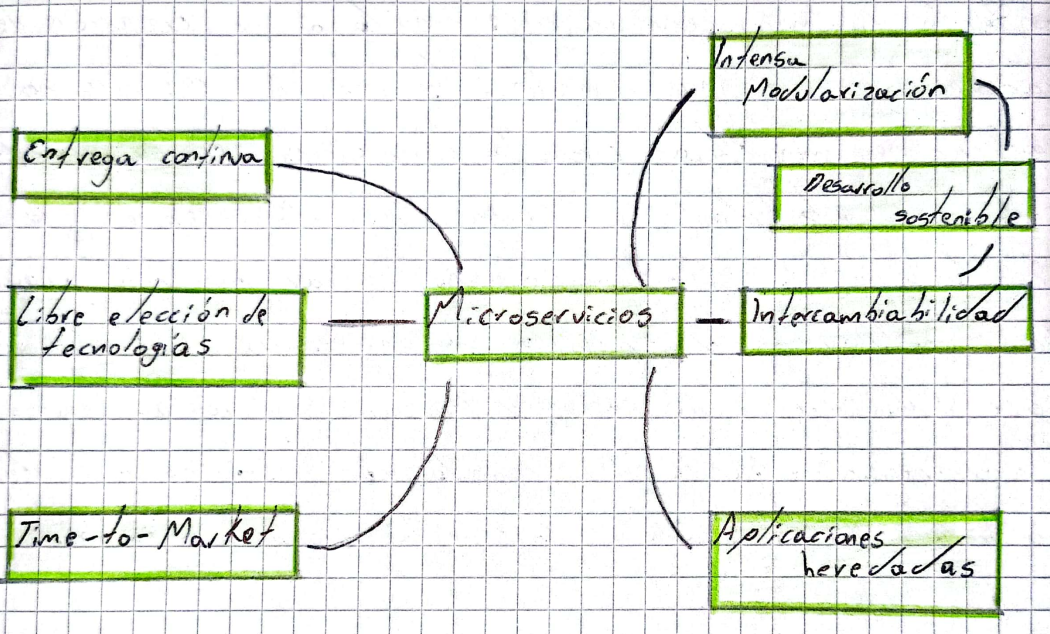
\includegraphics[scale=0.4]{microservicios.png} % Ajusta el tamaño con width
    \caption{Microservicios.}
    \label{fig:etiqueta-imagen} % Etiqueta para referenciar la imagen en el texto.
\end{figure}

\subsection{Mejora en la Calidad mediante Patrones de Diseño}
Los patrones de diseño, como el Observador y MVC, han
mostrado ser efectivos para estructurar sistemas sostenibles. En particular, el patrón MVC ha sido ampliamente utilizado en
aplicaciones móviles y web debido a su capacidad para separar
responsabilidades, facilitando el mantenimiento y la
escalabilidad. El uso de TDD en conjunto con patrones de
diseño, como se evidenció en el caso del SCACV, refuerza la
modularidad y reduce la probabilidad de errores.

\begin{figure}[H] % Utiliza [H] para que la imagen se coloque exactamente donde está el código.
    \centering
    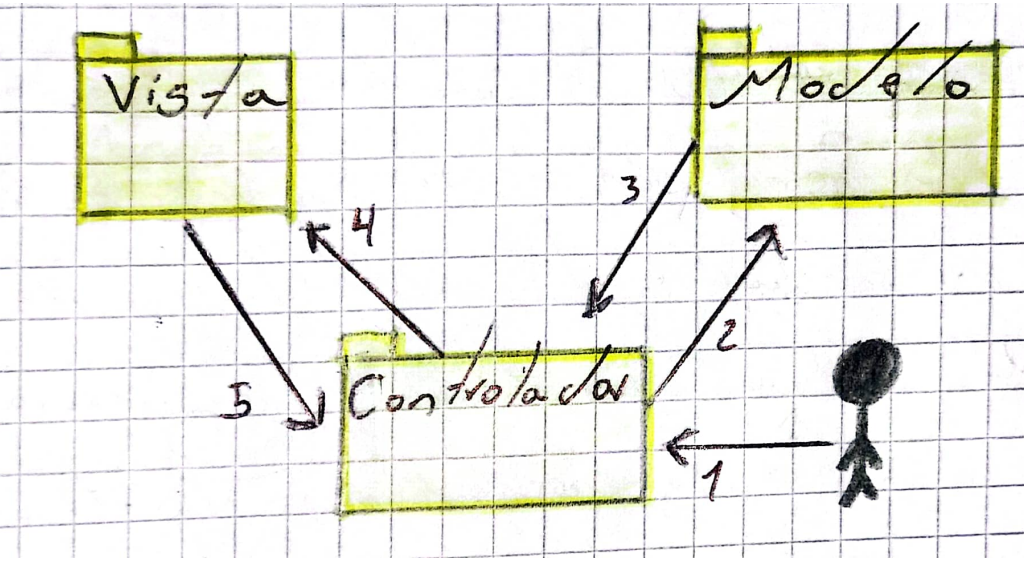
\includegraphics[scale=0.4]{mvc.png} % Ajusta el tamaño con width
    \caption{Modelo - Vista - Controlador.}
    \label{fig:etiqueta-imagen} % Etiqueta para referenciar la imagen en el texto.
\end{figure}

\subsection{Flexibilidad en la Gestión de Proyectos con Metodologías Ágiles}
Las metodologías ágiles, especialmente SCRUM y XP, han
demostrado su eficacia en la gestión de proyectos dinámicos.
La inclusión de un Sprint 0 para diseñar arquitecturas
preliminares ha permitido equilibrar la rapidez de la
metodología ágil con la necesidad de planificación
arquitectónica. Casos como el de sistemas de información
desarrollados bajo SCRUM muestran cómo este enfoque
mejora la comunicación entre los stakeholders y la capacidad
de adaptación a cambios.

\begin{figure}[H] % Utiliza [H] para que la imagen se coloque exactamente donde está el código.
    \centering
    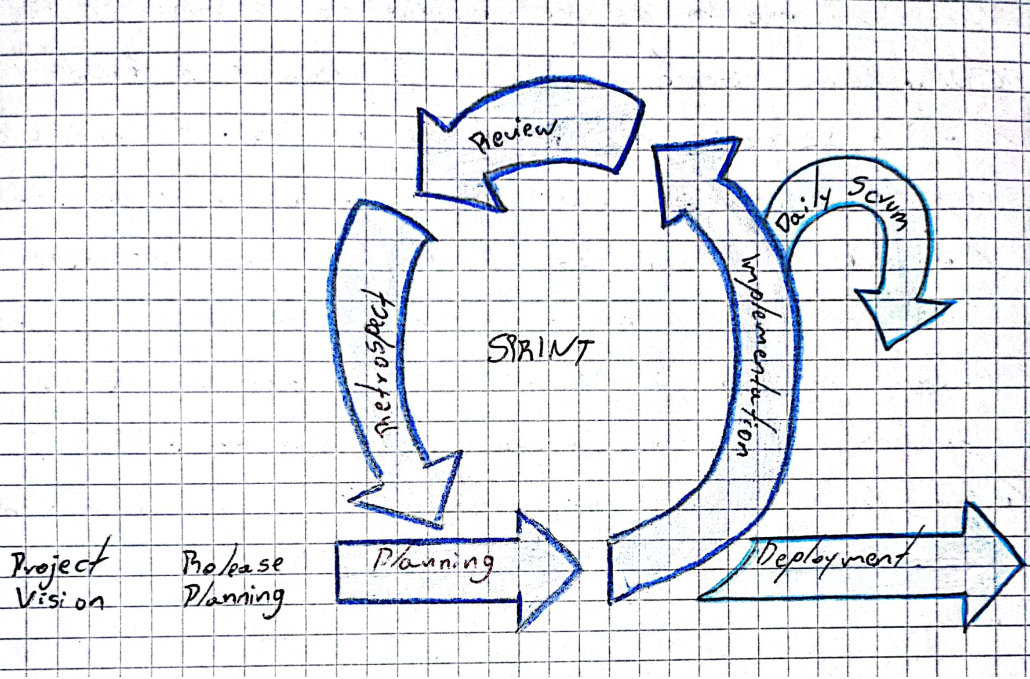
\includegraphics[scale=0.4]{scrum.png} % Ajusta el tamaño con width
    \caption{Proceso Scrum.}
    \label{fig:etiqueta-imagen} % Etiqueta para referenciar la imagen en el texto.
\end{figure}

\subsection{Evaluación de la Documentación y Métricas de Calidad}
La documentación adecuada, como se menciona en modelos como "Vistas y más allá" del SEI, es crucial para garantizar la trazabilidad en sistemas complejos. La herramienta SonarQube, utilizada en varios casos revisados, ha permitido identificar métricas de calidad clave, como la deuda técnica y la complejidad del código, mejorando la capacidad de mantenimiento.\\

\section{Discusión}
En esta sección se analizan los resultados obtenidos, comparándolos con estudios previos y destacando las contribuciones y limitaciones del enfoque propuesto. La integración de la arquitectura de software, los patrones de diseño y las metodologías ágiles representa un avance significativo en el desarrollo de sistemas modernos, pero también plantea desafíos que deben ser abordados.\\

\subsection{Análisis de Resultados}
Los resultados obtenidos reflejan que la combinación de arquitecturas robustas, como los microservicios y la arquitectura hexagonal, con metodologías ágiles, como SCRUM y XP, ofrece beneficios sustanciales en términos de escalabilidad, sostenibilidad y adaptabilidad. Este marco metodológico también evidencia que los patrones de diseño, como MVC y el Observador, no solo facilitan la estructuración de sistemas complejos, sino que, cuando se aplican junto con TDD, refuerzan la modularidad y reducen significativamente los errores.\\

Un hallazgo clave es que la inclusión de un Sprint 0 en SCRUM permite abordar una de las limitaciones más comunes en metodologías ágiles: la falta de planificación arquitectónica. Esto asegura que las decisiones arquitectónicas iniciales se documenten adecuadamente, mejorando la comunicación entre stakeholders y la adaptabilidad del sistema.

\subsection{Estudios Previos}
\begin{itemize}
    \item En el trabajo de la Asamblea Nacional del Ecuador, el uso de microservicios mostró beneficios similares en la escalabilidad y mantenimiento de sistemas distribuidos, reafirmando la eficacia de este enfoque.
    \item El caso del SCACV, que combinó patrones de diseño con TDD, también demostró cómo este enfoque mejora la calidad y cohesión del software, resultados que se alinean con nuestras observaciones.
    \item La propuesta de ICONIX como complemento a SCRUM, revisada en otros estudios, también se refleja en nuestros hallazgos, mostrando cómo puede equilibrarse la planificación arquitectónica con la flexibilidad de las metodologías ágiles.\\
\end{itemize}

\subsection{Limitaciones}
A pesar de los beneficios observados, el enfoque propuesto enfrenta algunas limitaciones:
\begin{itemize}
    \item Complejidad en la Integración: Combinar
    metodologías ágiles con planificación
    arquitectónica formal puede ser complejo y
    requiere experiencia previa en ambas disciplinas.
    Equipos sin formación en arquitectura de software
    podrían encontrar difícil implementar el Sprint 0 de
    manera efectiva.
    \item Demanda de Recursos: El uso de herramientas como
    UML y SonarQube, aunque valioso, puede no ser
    accesible para equipos pequeños o con recursos
    limitados
     \item Adaptación a Entornos Específicos: Si bien el marco
    es flexible, puede requerir ajustes significativos
    para proyectos con características únicas, como
    sistemas altamente regulados o de tiempo crítico.\\
\end{itemize}

\section{Conclusiones}
La integración de la arquitectura de software, los patrones de diseño y las metodologías ágiles representa un enfoque poderoso para abordar los desafíos del desarrollo de sistemas complejos en un entorno tecnológico en constante evolución. Este artículo ha analizado y propuesto un marco conceptual que equilibra la planificación arquitectónica con la flexibilidad ágil, ofreciendo beneficios significativos en términos de escalabilidad, calidad y adaptabilidad.\\

\subsection{Resumen de Hallazgo}
A lo largo del análisis, se ha demostrado que:
\begin{itemize}
    \item \textbf{Escalabilidad y Mantenimiento:} Las arquitecturas como los microservicios y la arquitectura hexagonal son esenciales para garantizar que los sistemas sean escalables y fáciles de mantener.
    \item \textbf{Calidad del Software:} Los patrones de diseño, en combinación con TDD, mejoran la modularidad y la calidad del código, reduciendo la incidencia de errores.
    \item \textbf{Gestión Ágil:} La inclusión de un Sprint 0 en SCRUM asegura que los proyectos comiencen con una base arquitectónica sólida, mitigando las limitaciones de la planificación insuficiente en metodologías ágiles tradicionales.
    \item \textbf{Documentación y Métricas:} Herramientas como UML y SonarQube no solo facilitan la documentación, sino que también permiten evaluar la calidad del software de manera objetiva, mejorando la trazabilidad y el control de riesgos.\\
\end{itemize}

\subsection{Implicaciones}
Estos hallazgos tienen importantes implicaciones para la industria del software:
\begin{itemize}
    \item La integración de estas disciplinas permite a las organizaciones responder a los cambios en los requisitos de manera más eficiente, asegurando al mismo tiempo la calidad y sostenibilidad del producto.
    \item En entornos académicos, el enfoque propuesto puede servir como modelo para enseñar a los estudiantes la importancia de equilibrar la planificación arquitectónica y la adaptabilidad ágil.
    \item En el sector empresarial, este marco puede aplicarse para optimizar la colaboración entre stakeholders y equipos de desarrollo, promoviendo una cultura de mejora continua y sostenibilidad a largo plazo.
\end{itemize}

\begin{thebibliography}{99}
\bibitem{blas2019} Blas, M. J., Leone, H. P., \& Gonnet, S. M. (2019). Modelado y Verificación de Patrones de Diseño de Arquitectura de Software para Entornos de Computación en la Nube.
\bibitem{sanabria2021} Sanabria, F. R., \& Rodríguez, S. V. (2021). Evaluación de una Arquitectura de Software. Prospectiva, 19(2).
\bibitem{cristia2021} Cristiá, M. (2021). Una Teoría para el Diseño de Software.
\bibitem{vera2023} Vera, J. B. V. (2023). Arquitectura de software con programación orientada a objeto. Polo del Conocimiento: Revista científico-profesional, 8(12), 1497-1508.
\bibitem{cambarieri2020} Cambarieri, M., Difabio, F., \& García Martínez, N. (2020). Implementación de una arquitectura de software guiada por el dominio. In XXI Simposio Argentino de Ingeniería de Software (ASSE 2020)-JAIIO 49 (Modalidad virtual).
\bibitem{guarin2023} Guarin, J. S. V. (2023). Especificando una arquitectura de software: Software architecture specification. Tecnología Investigación y Academia, 11(2), 170-181.
\bibitem{blancarte2016} Blancarte, O. (2016). Introducción a los Patrones de Diseño. México, México DF.
\bibitem{prieto2022} Prieto, C. A., \& Madrid, D. A. (2022). Buenas prácticas en la construcción de software: Best practices in software construction. Tecnología Investigación y Academia, 10(2), 149-166.
\bibitem{carignano2016} Carignano, M. C. (2016, June). Representación y razonamiento sobre las decisiones de diseño de arquitectura de software. In XVIII Workshop de Investigadores en Ciencias de la Computación (WICC 2016, Entre Ríos, Argentina).
\bibitem{perez2010} Pérez, J. S., Cuesta, C. E., \& Ossowski, S. (2010). El papel de las tecnologías del acuerdo en la definición de arquitecturas de software adaptativas. In Simposio Argentino de Ingeniería de Software (ASSE 2010)-JAIIO 39 (UADE, 30 de agosto al 3 de septiembre de 2010).
\bibitem{valbuena} Valbuena, D. C. Modelo de gestión de servicios PKI.
\bibitem{lopez2017} López, D., \& Maya, E. (2017). Arquitectura de Software basada en Microservicios para Desarrollo de Aplicaciones Web.
\bibitem{gonzalez2021} González-Castaño, L. E., Marroquín-Soto, S. V., Maturana-González, G. V., \& Manjarrés-Betancur, R. A. (2021). Coffee Challenge: Un juego para la enseñanza de patrones de diseño de software. Revista Politécnica, 17(33), 34-46.
\bibitem{capel} Capel, M. I., Grimán, A. C., \& Garví, E. Calidad Ágil: Patrones de Diseño en un contexto de Desarrollo Dirigido por Pruebas.
\bibitem{garnero} Garnero, A. B., \& Horenstein, N. Utilización de antipatrones y patrones en el análisis de software.
\bibitem{marticorena2002} Marticorena, R., López, C., García Osorio, C. I., \& Pardo, C. (2002). Aprendizaje práctico de patrones de diseño en asignaturas de programación de nivel III.
\bibitem{moreno2020} Moreno, J. C., Marciszack, M. M., \& Groppo, M. A. (2020). Patrones de Usabilidad Temprana en el Modelo Conceptual. AJEA, (5).
\bibitem{rojas2011} Rojas, M., \& Montilva, J. (2011). Una arquitectura de software para la integración de objetos de aprendizaje basada en servicios web. In Ninth LACCEI Latin American and Caribbean Conference. Engineering for a Smart Planet, Innovation, Information Technology and Computational Tools for Sustainable Development.
\bibitem{paez2018} Paez, A. H., Falcón, J. D., \& Cruz, A. A. P. (2018). Arquitectura de software para el desarrollo de videojuegos sobre el motor de juego Unity 3D. Revista de I+ D tecnológico, 14(1), 54-64.
\bibitem{gonzalez2020} González, J. E. F., \& García, C. A. O. Propuesta de diseño de arquitectura de software para la gestión, análisis y procesamiento de datos de neurociencia.
\bibitem{martin2012} Martín, Y. E. (2012). Arquitectura de software. Arquitectura orientada a servicios. Serie Científica de la Universidad de las Ciencias Informáticas, 5(1), 1-10.
\bibitem{sanchez2023} Sánchez, A. B., Parejo, J. A., Estrada-Torres, B., Márquez-Chamorro, A. E., del-Río-Ortega, A., \& Segura, S. (2023). Aprendiendo arquitectura software a partir de proyectos de código abierto en GitHub.
\bibitem{cortez} Cortez, A. A., \& Naveda, C. A. Una propuesta de implementación para especificaciones de patrones de comportamiento.
\bibitem{navarro2017} Navarro, M. E., Moreno, M. P., Aranda, J., Parra, L., Rueda, J. R., \& Pantano, J. C. (2017, September). Selección de metodologías ágiles e integración de arquitecturas de software en el desarrollo de sistemas de información. In XIX Workshop de Investigadores en Ciencias de la Computación (WICC 2017, ITBA, Buenos Aires).
\bibitem{astorga2019} Astorga, J. A. I., Tirado, J. L. O., Ramírez, R. U. R., Mendoza, J. C. L., \& Garzón, A. P. (2019). Clasificación de los patrones de diseño idóneos en programación Android. Revista Digital de Tecnologías Informáticas y Sistemas, 3(1).
\bibitem{vivas2013} Vivas, H. L., Cambarieri, M. G., García Martínez, N., Muñoz Abbate, H., \& Petroff, M. (2013). Un marco de trabajo para la Integración de Arquitecturas de Software con Metodologías Ágiles de Desarrollo.
\bibitem{granada2014} Granada, E. Z., Rodríguez, L. E. S., Montoya, C. E. G., \& Uribe, C. A. C. (2014). Arquitecturas de software para entornos móviles. Revista de Investigaciones Universidad del Quindío, 25(1), 20-27.
\bibitem{gomez} Gómez, O. Documentando la arquitectura de software.
\bibitem{moreno2003} Moreno, A. M., \& Sánchez-Segura, M. (2003, November). Patrones de Usabilidad: Mejora de la Usabilidad del Software desde el Momento Arquitectónico. In JISBD (pp. 117-126).
\bibitem{roque2015} Roqué Fourcade, L. E., \& Arakaki, L. (2015, May). Soporte a la actividad de diseño basado en patrones de diseño. In XVII Workshop de Investigadores en Ciencias de la Computación (Salta, 2015).
\bibitem{lund} Lund, M. I., Chavez, S. B., Ormeño, E. G., Martin, A., \& Matturro, G. MODELO DE CASOS DE USO. SU APLICACIÓN EN UN ENTORNO DE DESARROLLO GLOBAL DE SOFTWARE.
\bibitem{rodriguez} Rodríguez, I. Y. A., \& Cortes, E. E. P. R. Implementación de MVCC para la generación de Aplicaciones Web en tiempos de entrega reducidos.
\bibitem{arias2021} Arias-Orezano, J. F., Reyna-Barreto, B. D., \& Mamani-Apaza, G. (2021). Repercusión de arquitectura limpia y la norma ISO/IEC 25010 en la mantenibilidad de aplicativos Android. TecnoLógicas, 24(52), 226-241.
\bibitem{guevara} Guevara, W. J. T. Metodología para la enseñanza del Desarrollo de Software Modular.
\end{thebibliography}


\end{document}